\chapter{Crowdsourcing strategies in Pl@ntNet citizen based learning platform}
\label{chap:plantnet}
\enlargethispage{3\baselineskip}

\begin{keypointstwomargins}{Pl@ntNet}{-2cm}{-1cm}
        \textbf{Key points -- Crowdsourcing plant species}
        \begin{enumerate}[leftmargin=*]
        \item Aiding botanists in plant species identification is a challenging task. Species are often visually close and their identification requires expert knowledge.
        \item Pl@ntNet is a citizen science platform that allows users to upload images of plants and receive a list of possible species.
        \item The collaborative aspect of Pl@ntNet allows users to vote on the species they think are present in the image and contribute to new labeled data, which is then used to train a computer vision and help new identifications.
        \end{enumerate}

        \textbf{Contributions -- Exploration of Pl@ntNet label aggregation strategy}
        \begin{enumerate}[leftmargin=*,start=4]
        \item We release and evaluate the current Pl@ntNet label aggregation and compare it to other strategies.
        \item We release a subset of Pl@ntNet with images url and collected labels in the South Western European Flora of more than $6$ million observations and $800$ thousand users in a large-scale classification setting.
        \item We discuss how to integrate the current model's predictions in the votes aggregation. This is a challenging task due to the iterative aspect of Pl@ntNet: the current data helps train the next generation of models iteratively.
        \end{enumerate}
\end{keypointstwomargins}

\begin{figure}[thb]
        \centering
        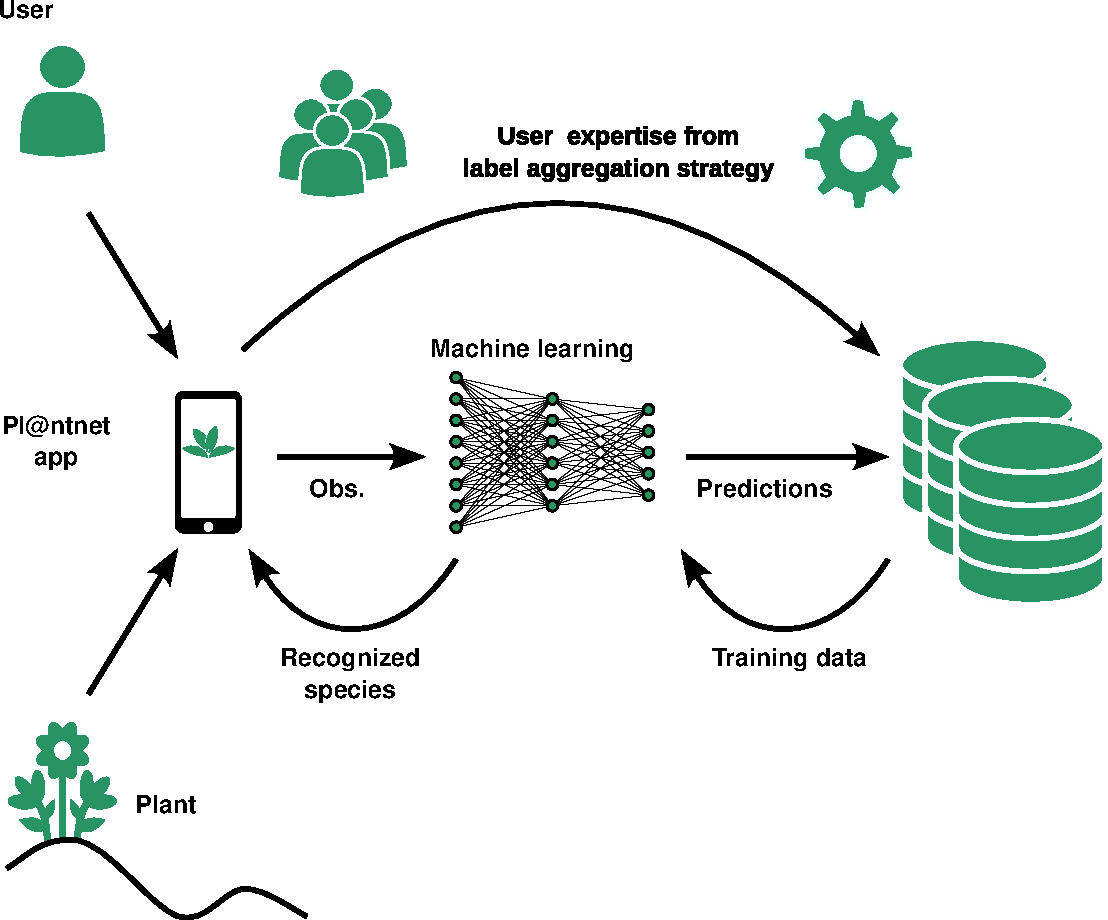
\includegraphics[width=.75\linewidth]{images/plantnet_schema_global_green.pdf}
        \caption{Pl@ntNet system of human-AI interaction for plant species recognition. Users take their plant observations in the Pl@ntNet application. A prediction is output by the AI model. Users can validate the prediction or propose another species. The whole votes collection is used to evaluate user expertise and actively revise observations identifications.}
        \label{fig:plantnet-system}
    \end{figure}


\section{Crowdsourcing for plant species identification}

Computer vision models are a great aid in plant species recognition in the field \citep{vidal2021perspectives,borowiec2022}.
However, to train them we need large annotated datasets.
These datasets are often created thanks to citizen science approaches, collecting both reliable and useful information \citep{brown2019potential}.
Among existing plant recognition applications, the Pl@ntNet citizen science platform \citep{affouard2017pl} enables global data collection by allowing users to upload and annotate plant observations.

\subsection{Plant taxonomy generalities}
First, we need to understand the complexity of plant taxonomy.
Our goal here is to briefly present the taxonomy of plants.
Plants are divided following a hierarchy, from the most general to the most specific ranks of taxa: kingdom, division, class, order, family, genus, and species according to the International Code of Nomenclature for algae, fungi and plants (ICN) \citep{turland2018international}.
Each of these units of biological classification is called a taxon (taxa in plural).
Further secondary ranks also exist (tribe, subspecies, variety, form) but we will focus on the main ones.

Roughly, an example of taxonomy levels is:
\begin{itemize}
        \item Kingdom: separates plants from animals, fungi, and bacteria -- \emph{e.g} Plantae.
        \item Division: separates spore (\emph{angiosperms}) or seed (\emph{gymnosperms}) reproduction with specific characteristics. There are 14 plant divisions in total.
        \item Class: Angiosperms are divided into Monocotyledons(grasses, yuccas, etc.) and Dicotyledons (angiosperms with pair of leaves).
        \item Order: Group of families with common characteristics -- \emph{e.g} \emph{Cucurbitales} (generally ends with \emph{-ales}).
        \item Family: Plants with similar flower, fruit and seed structures -- \emph{e.g} \emph{Begonaias and Allies}.
        \item Genus (genera in plural): First part of the plant's scientific name (capitalized and italicized) -- \emph{e.g} \emph{Begonia}.
        \item Species: a group of organisms capable of producing fertile offspring -- \emph{e.g} \emph{Begonia ferox}. If the species is unknown it is called \emph{sp.} or \emph{spp.} for plural.
\end{itemize}

In the case a plant is a hybrid -- a cross between two species -- it is written with an x as in \emph{Begonia} x \emph{semperflorens}. The position of the x indicates if it is the hybridization between two genera or species.
For example, the × \emph{Agroelymus hajastanica} is the hybridization of the \emph{Agropyron cristatum} and the \emph{Elymus repens} -- note that the genera are aggregating into a resulting genus.
Similarly to the x, a + is used to indicate a transplant chimera between two plants.
For example, the + \emph{Laburnocytisus adamii} results of the transplant of two individuals with different genera: the \emph{Laburnum anagyroides} and the \emph{Cytisus purpureus}.


\subsubsection{Checklists and referentials}

The plant name is generally composed of only two parts: the genus and the species.
Botanists have created checklists of accepted plant species.

One of the largest is the International Plant Names Index (IPNI) \citep{IPNI2024}.
The IPNI is a database of the published names and indicates which names are validly published.
It does not take into account the taxonomic status of the names -- the chronological changes and synonymity.
The World Checklist of Vascular Plants (WCVP) \citep{govaerts2021world} is an international collaborative database of taxa that provides the latest nomenclatural and taxonomic information on vascular plants -- \emph{clubmosses}, \emph{horsetails}, \emph{ferns}, \emph{gymnosperms} (including conifers), and \emph{angiosperms} (flowering plants).
The data from WCVP is the backbone for Plants Of the World Online (POWO) \footnote{\url{https://powo.science.kew.org}} which is an interface to access more information on individual species as their distribution for example.

There are multiple other checklists and databases such as The Plant List (TPL) \citep{PlantList2013}, the Catalogue of Life (CoL) \citep{cachuela2006towards}, Leipzig Catalogue of Vascular Plants (LCVP) \citep{freiberg2020leipzig} \emph{etc.} For a more exhaustive comparison of these databases we refer the reader to \citet{schellenberger2023big}.
The Global Biodiversity Information Facility (GBIF) \citep{telenius2011biodiversity} is an openly accessible network of shared knowledge about biodiversity on Earth.
They currently regroup $105$ different sources of taxonomy\footnote{\url{https://www.gbif.org/fr/dataset/d7dddbf4-2cf0-4f39-9b2a-bb099caae36c}}.

These checklists are the backbone of any botanical project as they provide a reference for the species names, their taxonomic status, and synonymic contributions.
Synonyms are not rare in plant taxonomy and can be due to different reasons such as the same species being described by different botanists, at different times, in different regions of the world.
As an example, in WCVP there are $357347$ plant species and $565200$ synonyms for those species.

Moreover, note that checklists might not always cover all the species and synonyms from one another.
For example, the \emph{Pilosella officinarum Vaill.} is listed in POWO with $161$ possible synonyms  -- $141$ accepted synonyms and $20$ illegitimate -- while in the GBIF it is listed with $241$ possible synonyms.
In the Pl@ntNet database, synonyms are only considered at the species level, resulting in $22$ possible accepted synonyms for this species.

\subsection{What is a plant observation?}

Contrary to classical datasets, Pl@ntNet observations are not a single image but a set of images taken by a user in the field.
A single image of a plant might not be enough to identify the species.
More images of different parts of the plant -- leaves, flowers, fruits, \emph{etc.} -- are needed to correctly identify the species and mimic a botanist's behavior while it is surely not the same and we can not replace such expertise.

In the field, some recommendations include\footnote{\url{https://ibis.geog.ubc.ca/biodiversity/eflora/identification.html}} but are not limited to:
\begin{itemize}
        \item the type of plant: a shrub, an herb, a fern, \emph{etc.}
        \item physical traits of the plant -- height, color range, hairy (length, width), texture (velvety, rough, smooth), is it stingy, thorny? \emph{etc.}
        \item position and number of leaves, flowers (symmetrical, shape), fruits or seeds (size, flesh), \emph{etc.}
        \item blooming period
        \item the aroma (minty, pungent)
        \item grown habits -- bushy, sprawling around, erected, vine-like
        \item \dots
\end{itemize}

Once these criteria are gathered, the botanist can identify possible species.
To filter out the possible species, the botanist will also consider the habitat -- sand, marshes, rocky fields -- the elevation -- sea level, mountain -- and the region to narrow the confusion.

Most of these criteria (like the aroma, texture or habitat), can be difficult or even impossible yet to be gathered from multiple images, and much less from a single one.
Hence, the use of multiple images is crucial to correctly identify the species or at least narrow down the possible species.
Botanists will observe multiple organs (flower, fruit, leaf), from different angles (a flower from the bottom view can have specific traits not visible from the side).
These characteristics can be transmitted via multiple images for the same observation.


\subsection{Presenting the voting interface}

\subsection{A step in a bigger pipeline}

\section{Pl@ntNet's label aggregation strategy}

\subsection{Presentation of the algorithm}

\subsection{Introducing a subset of Pl@ntNet to evaluate the current strategy}

\section{Integrating model predictions in the aggregation}

\subsection{Possible strategies}

\subsection{Can we trust our current predicted probabilities?}

\section{Conclusion}